\documentclass{beamer}
\mode<presentation>
\usetheme{Madrid}
\usecolortheme{crane}

\usepackage{tikz}
\usepackage{epic}
\usepackage{tikz-qtree}
\usepackage{linguex}
\usepackage[normalem]{ulem}
\usepackage{tikz-dependency}
\usepackage{colortbl}
\usepackage{xcolor}
\definecolor{darkgreen}{rgb}{0,0.3,0}
\definecolor{darkblue}{rgb}{.05,.05,.30}
\definecolor{lightgrey}{rgb}{0.65,0.65,0.65}
\usepackage{tikzsymbols}
\usepackage{amsmath}

\usepackage{verbatim}
\usepackage{setspace}
\usepackage{graphbox}
\usepackage{url}
\usetikzlibrary{matrix,arrows,positioning,automata,shadows,shapes.geometric,shapes.misc}


\DeclareMathOperator*{\argmax}{argmax}

\newcommand{\actfun}[1]{\includegraphics[height=0.11\textheight,align=c]{../images/#1}} % For consistency

\newcommand{\norm}[1]{\left\lVert#1\right\rVert}
\newcommand{\remph}[1]{\textbf{\color{red} #1}}

\newcommand{\teeny}[1]{\scalebox{0.17}{#1}}
\newcommand{\tablecolors}{\rowcolors{2}{blue!12}{white}} % Cool table colors
\newcommand{\detail}[1]{{\color{lightgrey}\small{}#1}}

\title[LT2222 lecture 4]{LT2222 Machine learning for statistical NLP: intro, Winter 2021}
\subtitle{Lecture 4: Neural networks; gradient descent; more softmax}
\author[Sayeed]{Asad Sayeed\\{\small (with some content from Jon Dehdari\\{\tt https://github.com/jonsafari/lt1/})}}
\institute[Gothenburg]{University of Gothenburg}
\date{}

\setbeamertemplate{navigation symbols}{}

\newcommand{\placard}[1]{
  \begin{frame}
    \begin{center}
      \huge
      \textbf{#1}
    \end{center}
  \end{frame}
}

\newcommand{\pagestep}[2]{
  \begin{frame}[t]
    \begin{minipage}[t][0.26\textheight][t]{\textwidth}
      \begin{center}
        \huge
        \textbf{#1}
      \end{center}
    \end{minipage}
    
    \begin{minipage}[t][0.7\textheight][c]{\textwidth}
      \begin{center}
        \includegraphics[height=0.83\textheight]{#2}
      \end{center}
    \end{minipage}
  \end{frame}
}

\newcommand{\pagestepalt}[2]{
  \begin{frame}[t]
    \begin{minipage}[t][0.26\textheight][t]{\textwidth}
      \begin{center}
        \huge
        \textbf{#1}
      \end{center}
    \end{minipage}
    
    \begin{minipage}[t][0.7\textheight][c]{\textwidth}
      #2
    \end{minipage}
  \end{frame}
}

%% \newcommand{\pagestepaltfragile}[2]{
%%   \begin{frame}[fragile][t]
%%     \begin{minipage}[t][0.26\textheight][t]{\textwidth}
%%       \begin{center}
%%         \huge
%%         \textbf{#1}
%%       \end{center}
%%     \end{minipage}
    
%%     \begin{minipage}[t][0.7\textheight][c]{\textwidth}
%%       #2
%%     \end{minipage}
%%   \end{frame}
%% }


\begin{document}
\makeatletter
\setbeamertemplate{footline}
{
  \leavevmode%
  \hbox{%
  \begin{beamercolorbox}[wd=.333333\paperwidth,ht=2.25ex,dp=1ex,center]{author in head/foot}%
    \usebeamerfont{author in head/foot}\insertshortauthor\expandafter\beamer@ifempty\expandafter{\beamer@shortinstitute}{}{~~(\insertshortinstitute)}
  \end{beamercolorbox}%
  \begin{beamercolorbox}[wd=.333333\paperwidth,ht=2.25ex,dp=1ex,center]{title in head/foot}%
    \usebeamerfont{title in head/foot}\insertshorttitle
  \end{beamercolorbox}%
  \begin{beamercolorbox}[wd=.333333\paperwidth,ht=2.25ex,dp=1ex,right]{date in head/foot}%
    \usebeamerfont{date in head/foot}\insertshortdate{}\hspace*{2em}
%    \insertframenumber{} / \inserttotalframenumber\hspace*{2ex} 
    \insertframenumber{}\hspace*{2ex}
    \hspace*{6ex}
  \end{beamercolorbox}}%
  \vskip0pt%
}
\makeatother


\begin{frame}
  \titlepage
\end{frame}

\pagestepalt{Today's agenda:}{
  \begin{enumerate}
  \item Basics of feed-forward neural networks
  \item Basics of stochastic gradient descent
  \item A little more on softmax
  \end{enumerate}
}

\placard{Part 1: Basic feed-forward neural networks}

\pagestepalt{Maximum entropy again}{
  \begin{block}{}
    \begin{center}
      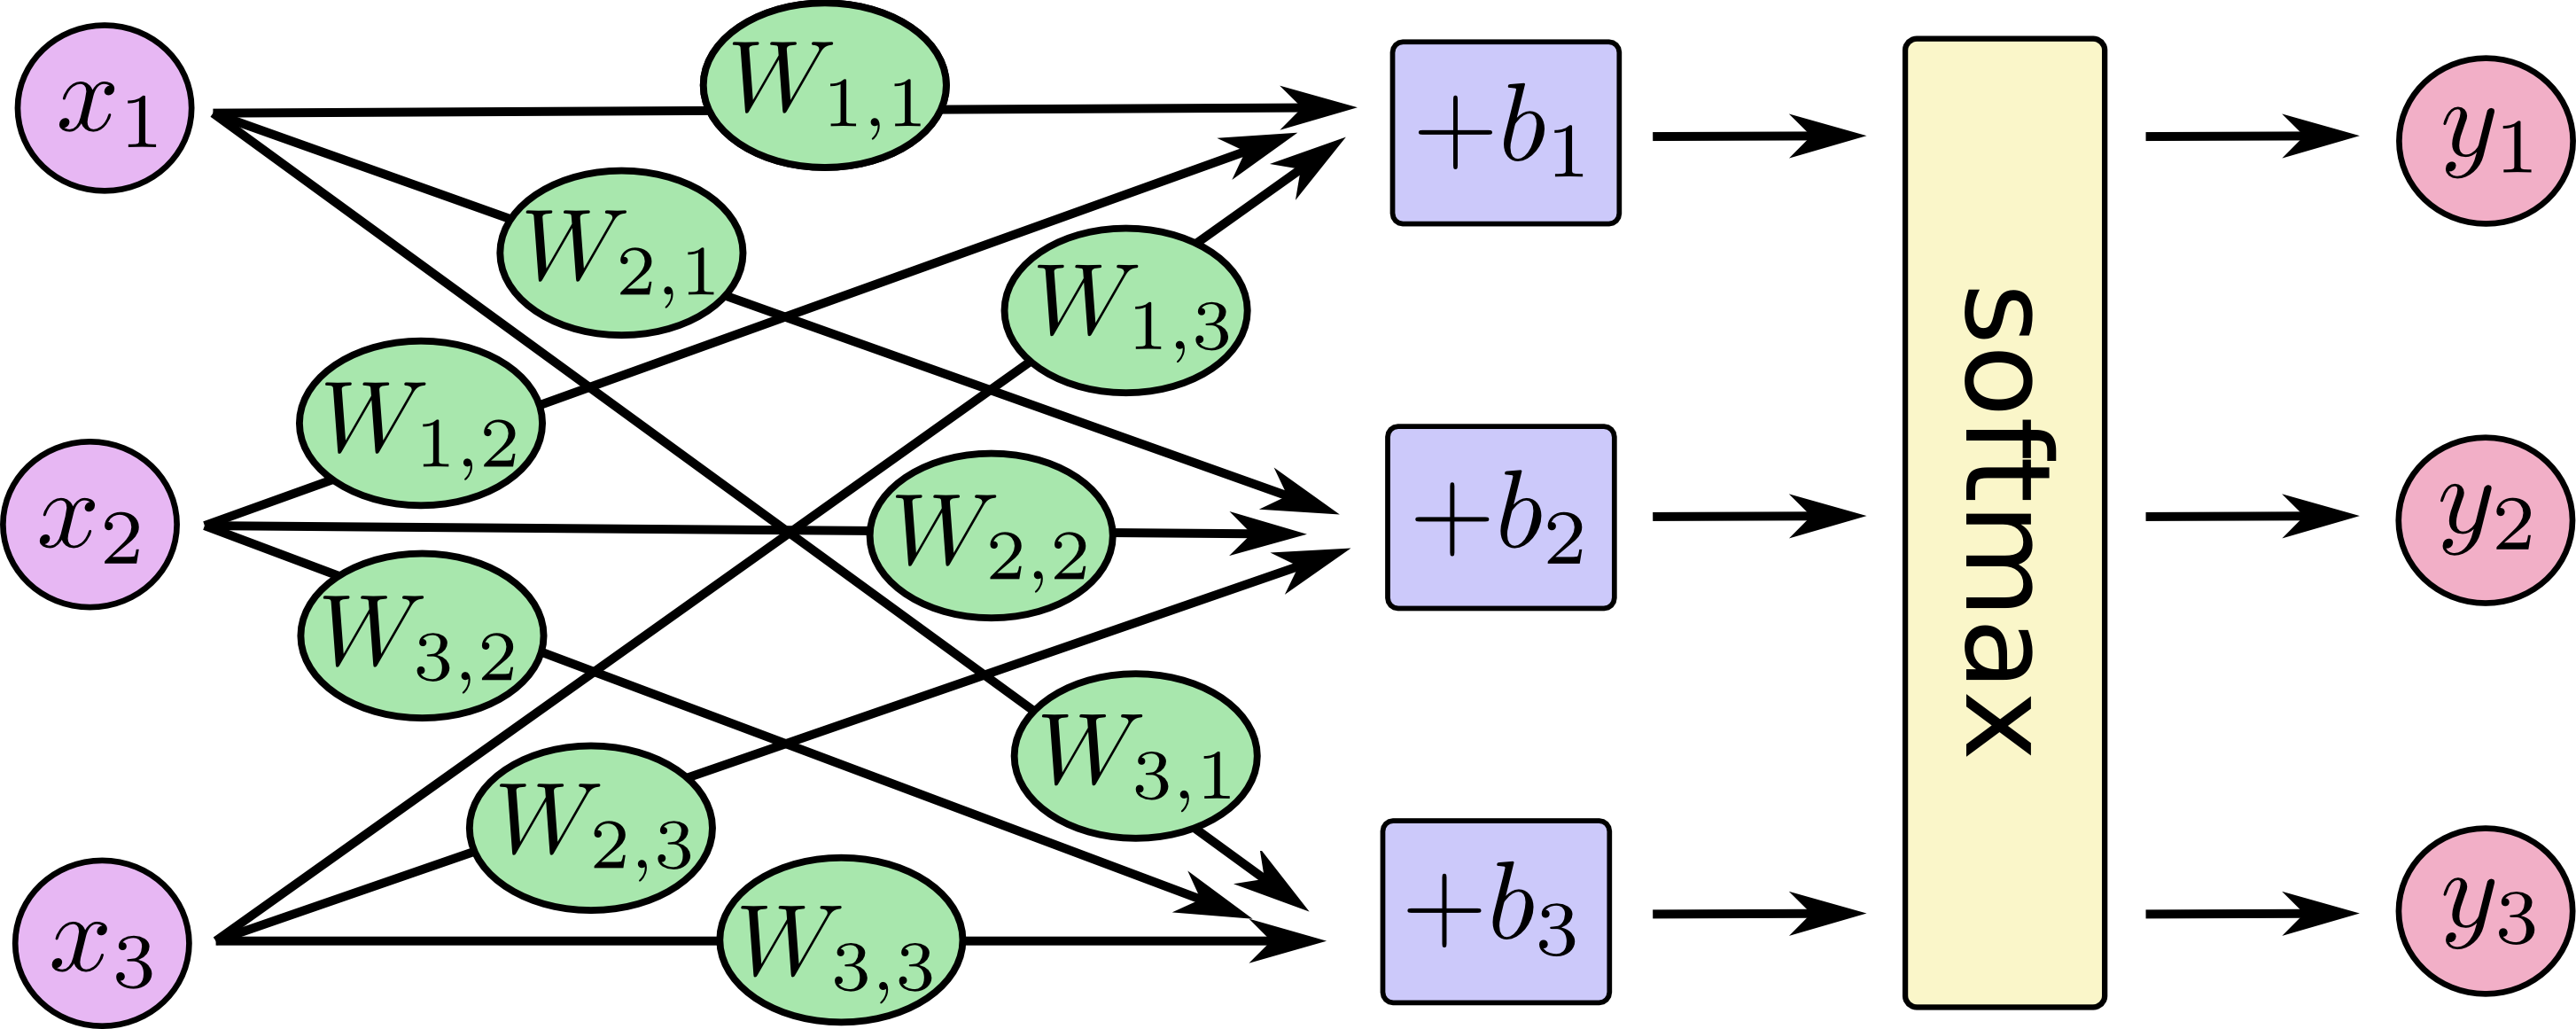
\includegraphics[height=0.29\textheight]{../images/softmax-regression-scalargraph.png}
    \end{center}
  \end{block}\pause
  Another way to think of the bias term is that we set one input
  neuron $x_n$ to $1.0$ permanently.\\\pause
  Finding the weight matrix $\mathbf{W}$ involves numerical optimization
  tricks we won't get into, but one possibility is a form of gradient descent.
  {\tiny Courtesy of
    \href{http://www.tensorflow.org/tutorials}{TensorFlow}}
}


\pagestepalt{Extending softmax regression}{
  \vspace{-0.2cm}
  \begin{itemize}
  \item {\small Recall that \textbf{logistic regression} involves the dot product of an input vector and a weight matrix, then a normalized sigmoid function (softmax)}
    \pause
  \item A \textbf{feedforward neural network} just adds one or more layers between the input vector and the softmax output
    \pause
    \begin{center}
      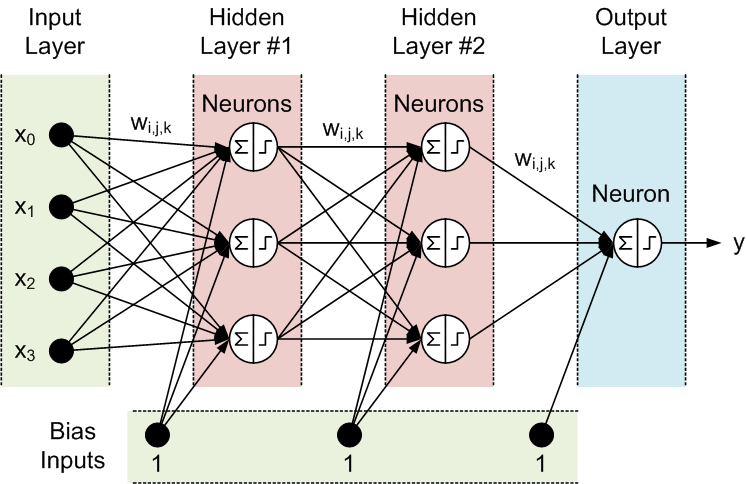
\includegraphics[height=0.5\textheight]{../images/nnet_mql5.png}
    \end{center}
  \end{itemize}
  \teeny{Courtesy of \href{https://www.mql5.com/en/code/9002}{mql5.com}}
}

\pagestepalt{Why use hidden layers?}{
  \vspace{-0.3cm}
  \begin{itemize}
  \item In contrast to log-linear models, neural networks can have \textbf{non-linear} representations of data\pause
  \item The \textbf{\href{https://en.wikipedia.org/wiki/Universal_approximation_theorem}{universal approximation theorem}} (George Cybenko, 1989) found that a neural network with one hidden layer can approximate \textbf{any continous function}\pause
  \item A network with two hidden layers can represent discontinuous functions\pause
    \begin{center}
      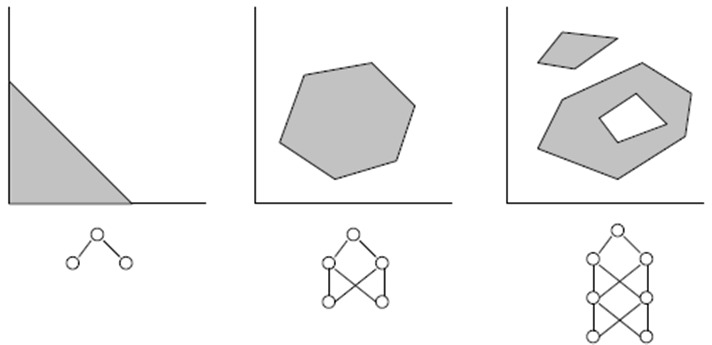
\includegraphics[height=0.35\textheight]{../images/nnet_mql5_function_approximations.png}
    \end{center}
  \end{itemize}
  \vspace{-0.3cm}
  \teeny{Courtesy of \href{https://www.mql5.com/en/code/9002}{mql5.com}}
}

\pagestepalt{Activation Functions ($\sigma$)}{
  \vspace{-0.8cm}
  In each layer, the output of the dot product goes through an \textbf{\href{https://en.wikipedia.org/wiki/Activation_function}{activation function}} ($\sigma$). Here are some examples: \\
  \vspace{-1em}

  %\scalebox{0.8}{
\begin{footnotesize}
\begin{spacing}{0.85}
  %\hspace*{-3.0em}%
  \scalebox{0.8}{
\begin{tabular}{lllp{0.38\textwidth}}
	\bf Name & \bf Visualization & $\bf f(x)=$ & \bf Notes \\
	\hline
	Linear  (= Identity) & \actfun{activation_linear_wp.png} & $x$ & Not useful for hidden layers \\
	Heaviside Step & \actfun{activation_heaviside_step_wp.png} & {\tiny $ \left \{\begin{array}{rcl} 0 & \mbox{if} & x < 0\\ 1 & \mbox{if} & x \ge 0\end{array} \right. $ }  \hspace*{-1.0em} & Not differentiable \\
{\scriptsize Rectified Linear (ReLU)} & \actfun{activation_relu_wp.png} & {\tiny $ \left \{\begin{array}{rcl} 0 & \mbox{if} & x < 0 \\ x & \mbox{if} & x \ge 0\end{array} \right.$ } \hspace*{-1.0em} & Surprisingly useful in practice \\
	Tanh & \actfun{activation_tanh_wp.png} & $\frac{2}{1+e^{-2x}}-1$ & A soft step function; ranges from -1 to 1 \\
	Logistic (`sigmoid') & \actfun{activation_logistic_wp.png} & $\frac{1}{1+e^{-x}}$ & Another soft step function; ranges from 0 to 1 \\
	Softmax & \actfun{activation_logistic_wp.png} & $\frac{e^{\boldsymbol W_y \cdot \mathbf{x}} }{Z} $ & Normalized sigmoidal function. Useful for last layer when training on cross entropy \\
\end{tabular}
}
\end{spacing}
\end{footnotesize}
%}
\pause
\vspace{-0.1cm}
    {\tiny \href{http://keras.io/activations}{List of activation functions in Keras: \texttt{keras.io/activations}}}\\
    \vspace{-0.3cm}
\teeny{Images courtesy of \href{https://en.wikipedia.org/wiki/Activation_function}{Wikipedia}}
}

\pagestepalt{Training Neural Networks}{
\begin{itemize}
	\item At a high level, the weights in a neural net are set by means of the blame game -- whenever it guesses incorrectly, change the weights that were the most responsible for making that guess
	\pause
	\item Whenever the network guesses a training instance correctly, don't change anything
	\pause
	\item The weights are usually trained by a form of the gradient descent optimization algorithm
	\item The gradients are calculated by error \textbf{backpropagation}
	\item First, do a normal forward pass through the network, to determine the \textbf{error/loss} (how different the output was from the `correct' answer)
	\item Then, do a backwards pass (end to start), changing the weights to minimize errors
\end{itemize}
}

\pagestepalt{Loss / Objective Functions}{
\begin{itemize}
	\item \textbf{Discrete Outputs}:
	\begin{itemize}
		\item Binary Cross-Entropy (0-1 loss): 0 if correct, 1 if incorrect
		\item Categorical Cross-Entropy: good old cross-entropy. Eg.\\ 0 if $p(y)=1.0$, \\ 1 if $p(y) = 0.5$, \\ 2 if $p(y)=0.25$, \\ 3 if $p(y)=0.125$, \\ ...
	\end{itemize}
	\item \textbf{Continuous Outputs}:
	\begin{itemize}
		\item Mean Squared Error (MSE): $\frac{1}{n} \sum_{i=1}^n (\hat{y}_i - y_i)^2$
		\item Root Mean Squared Error (RMSE): $\sqrt{MSE}$
		\item Mean Absolute Error (MAE): $\frac{1}{n} \sum_{i=1}^n |\hat{y}_i - y_i|$
	\end{itemize}
\end{itemize}
\pause
\vspace*{1.0em}
\href{http://keras.io/objectives}{List of loss functions in Keras: \texttt{keras.io/objectives}}
}

\pagestepalt{Autoencoders}{
\begin{itemize}
	\item An \textbf{autoencoder} is a neural network where the size of the output layer is the same size as the input layer
	\item The hidden layers are usually smaller
	\item The goal is to generalize the training data
	\item Since no labeled data is necessary, autoencoders are an unsupervised learning technique
	\item Autoencoders trained on language data are neural language models
	\pause
	\item Autoencoders are occasionally called \href{https://en.wikipedia.org/wiki/Diabolo\#History_and_etymology}{diabolo networks} \\
	\begin{center}
		\href{https://www.youtube.com/watch?v=x_TSOi2aQUM}{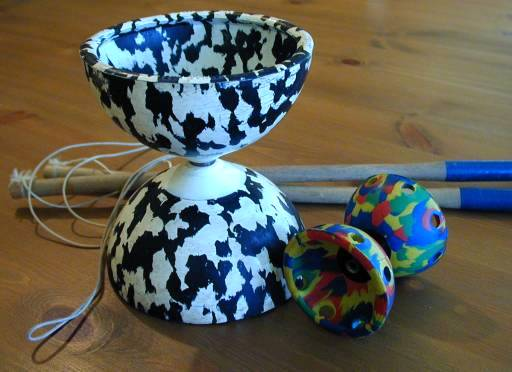
\includegraphics[height=0.35\textheight]{../images/diabolo_large_and_small.jpg}}
	\end{center}
\end{itemize}
\teeny{Image courtesy of \href{https://commons.wikimedia.org/wiki/File:Diabolo_large_and_small.jpg}{Wikimedia}}
}

\placard{Part 2: Basics of stochastic gradient descent}

\pagestepalt{From curves to derivatives}{
  There's a way to ``find'' a derivative that's an extension of the way
  to calculate slope. For function $f(x)$
  \begin{block}{}
    \[\frac{df(x)}{dx} = \lim_{\Delta x \rightarrow 0} \frac{f(x + \Delta x) - f(x)}{\Delta x}\]
  \end{block}
  \begin{itemize}
  \item Taking $m =\frac{\Delta y}{\Delta x}$ as with the linear function
    $y=mx+b$, is just a special,
    simple case of taking $\frac{df(x)}{dx}$. \pause
  \item For a function $F$ over a vector $\mathbf{x}$, we have to take
    ``partial derivatives'' (over each dimension), and we write that as $\nabla F(\mathbf{x}) = (\frac{\partial F}{\partial x_0} \ldots \frac{\partial F}{\partial x_n})$.
  \end{itemize}
}

\pagestepalt{Finding the weights}{
  \vspace{-0.2cm}
  \begin{columns}[T]
    \begin{column}{0.49\textwidth}
      \begin{center}
  %      \uncover<1>{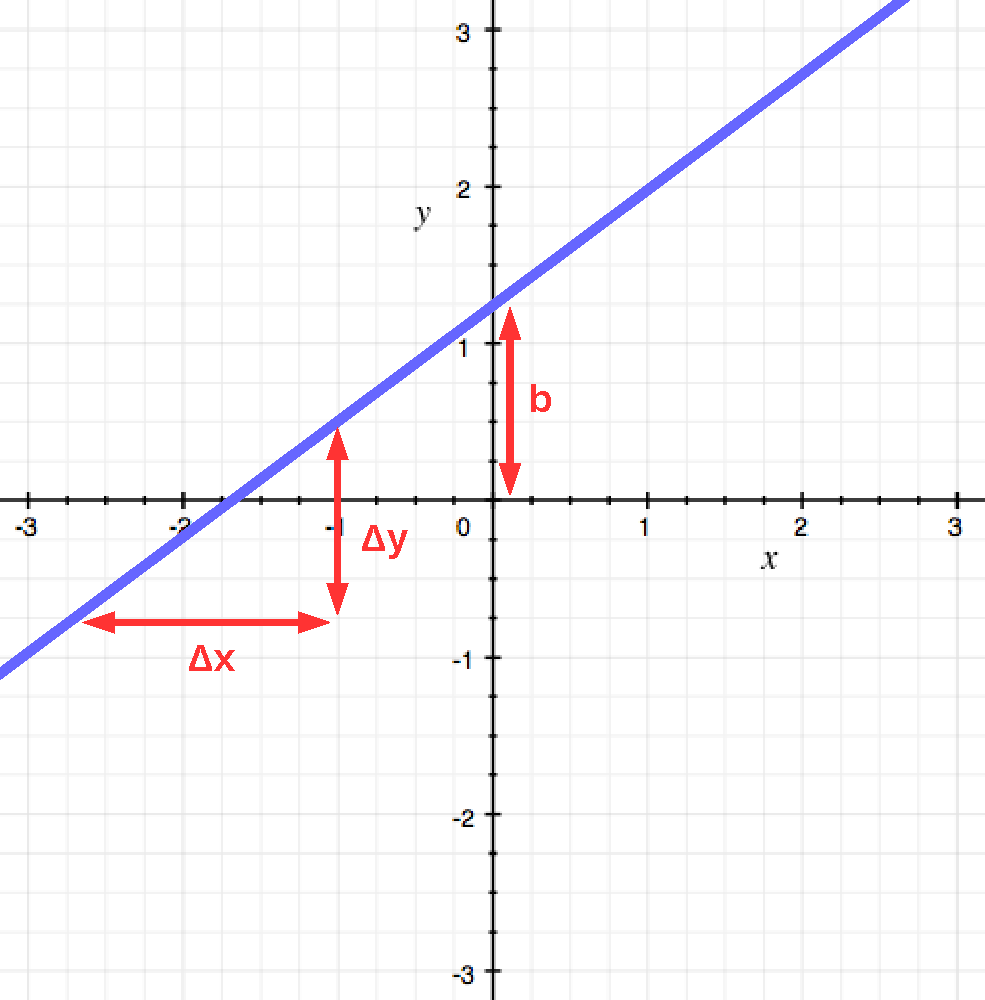
\includegraphics[width=0.9\textwidth]{cart4.pdf}}
  %      \uncover<2>{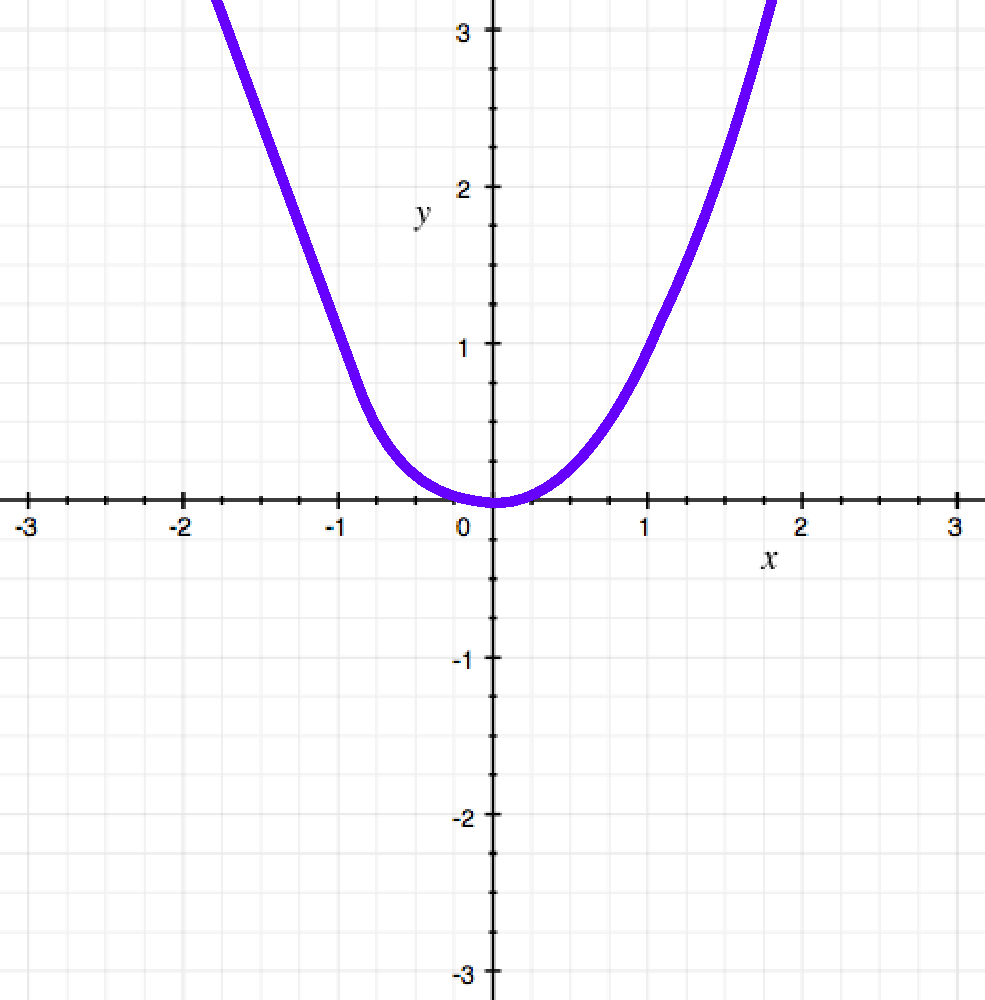
\includegraphics[width=0.9\textwidth]{quad0.pdf}}
  %      \includegraphics<3>[width=0.9\textwidth]{quad1.pdf}
        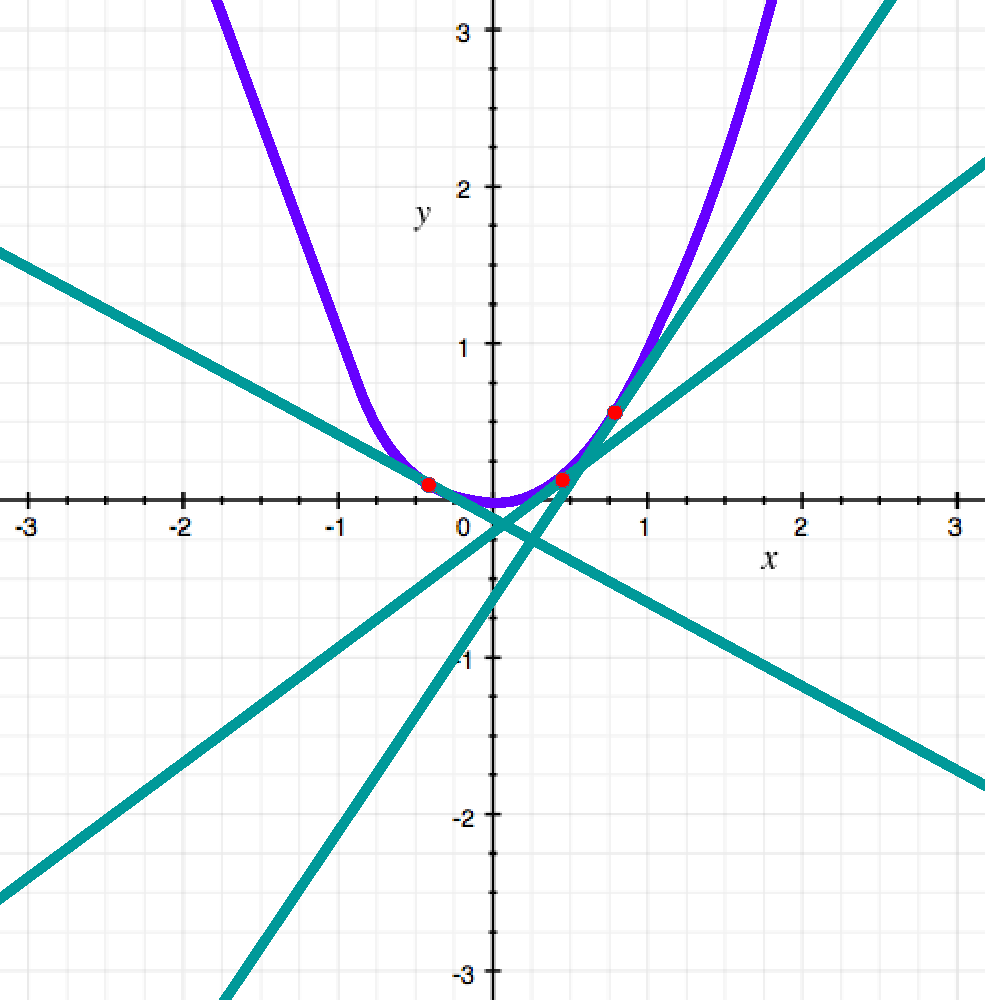
\includegraphics[width=0.9\textwidth]{quad2.pdf}
      \end{center}
    \end{column}
    \begin{column}{0.49\textwidth}
      \begin{itemize}
      \item Linear classification: finding the weights that describe a
        separating plane.\pause
      \item The weights define the slope of a plane in a
        high-dimensional space.\pause
      \item Problem is, the weights themselves must be found in a
        space \ldots that is not necessarily linear (ie, the space
        representing your problem).\pause
      \item So if your problem space is defined by $F(\mathbf{x})$, then
        you're looking for weights in $\nabla F(\mathbf{x})$\ldots
      \end{itemize}
    \end{column}
  \end{columns}
}

\pagestepalt{``Vanilla'' gradient descent}{
  \vspace{-0.2cm}
  \begin{columns}[T]
    \begin{column}{0.49\textwidth}
      \begin{center}
  %      \uncover<1>{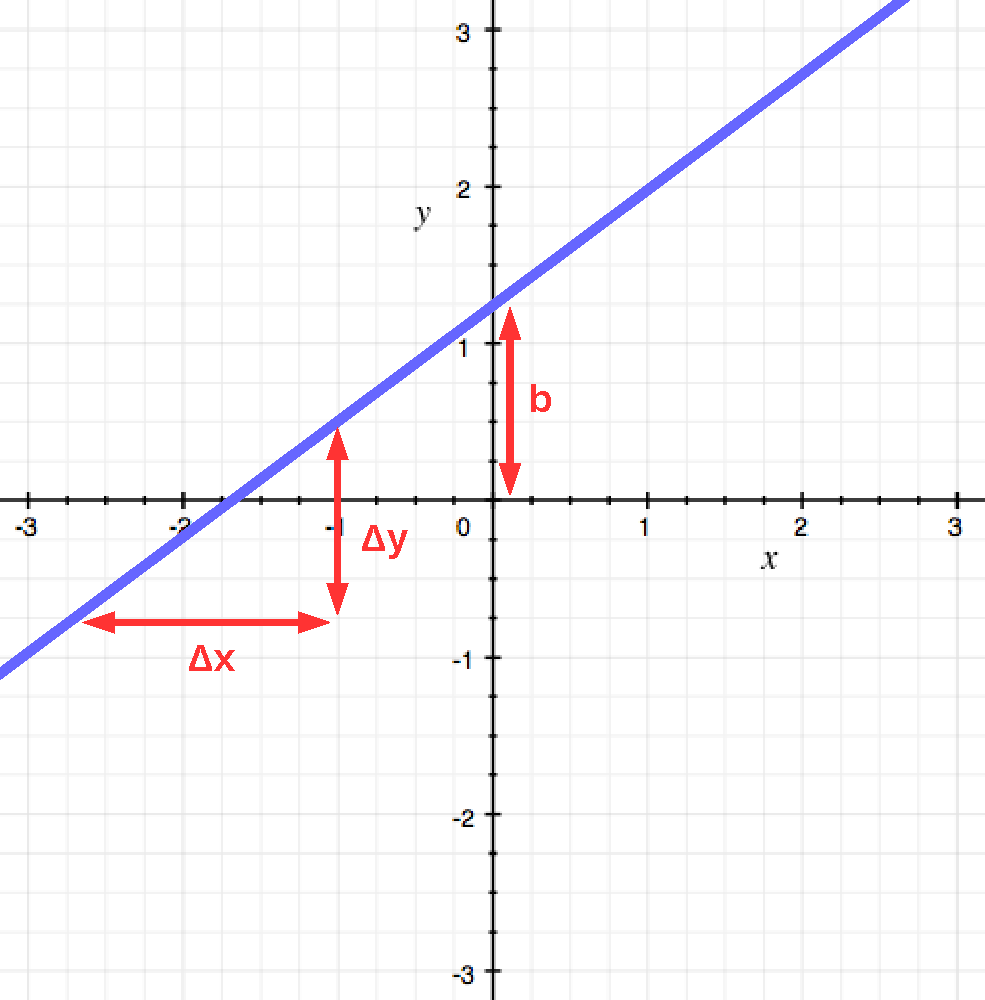
\includegraphics[width=0.9\textwidth]{cart4.pdf}}
  %      \uncover<2>{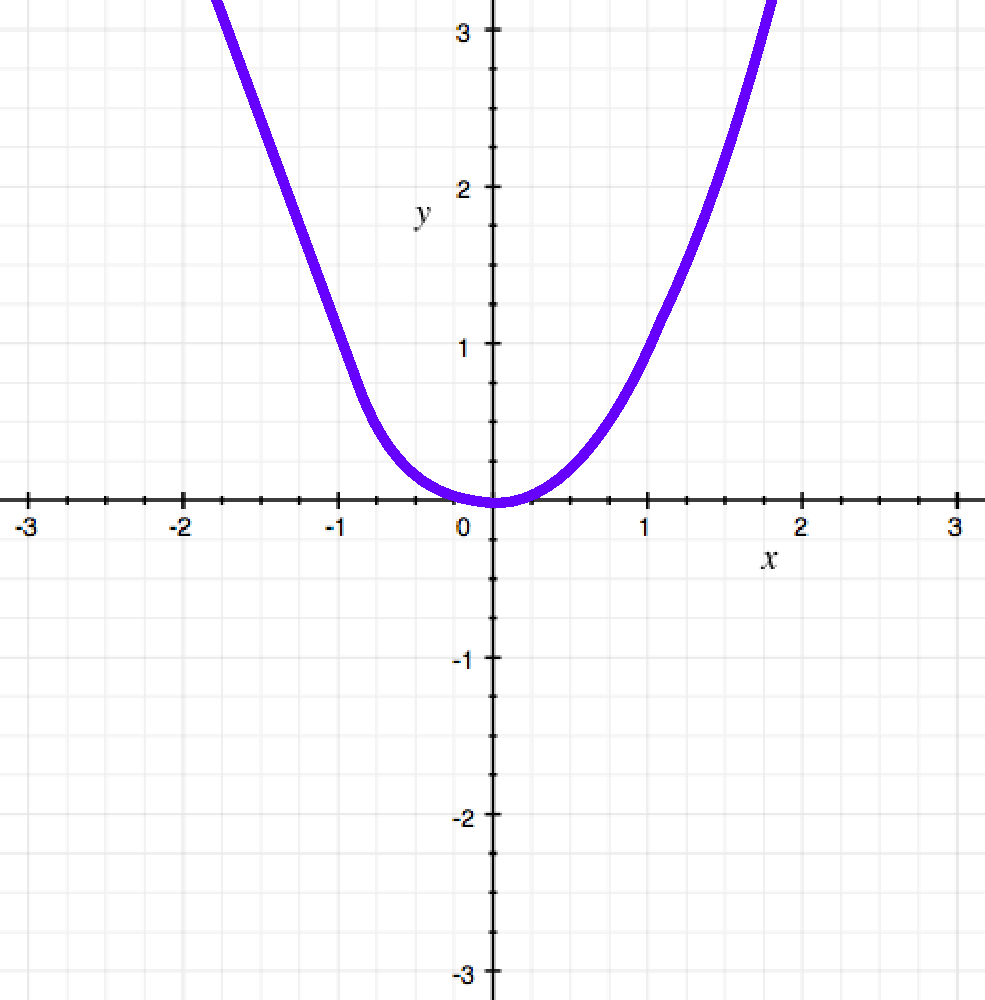
\includegraphics[width=0.9\textwidth]{quad0.pdf}}
        %      \includegraphics<3>[width=0.9\textwidth]{quad1.pdf}
        (from Wikipedia)\\
        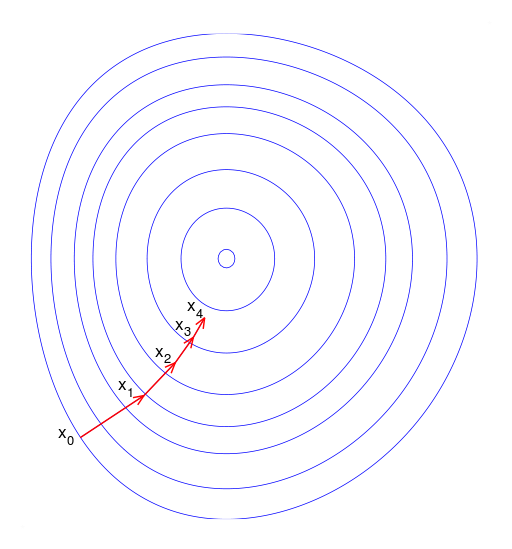
\includegraphics[width=0.9\textwidth]{grad0.png}
      \end{center}
    \end{column}
    \begin{column}{0.49\textwidth}
      Assume your objective
      function $F(\mathbf{x})$ is ``defined and differentiable'' at point
      $\mathbf{a}$.\\\pause
      \begin{itemize}
      \item Find a ``lower'' point than $\mathbf{a}$ by following the
        negative slope $-\nabla F(\mathbf{a})$
        \begin{block}{}
          \[\mathbf{a}_{n+1} = \mathbf{a}_n - \gamma \nabla F(\mathbf{a}_n) \]
        \end{block}\pause
      \item If we can keep changing $\gamma$ between steps, we can guarantee
        \alert{convergence}.
      \end{itemize}
    \end{column}
  \end{columns}
}

\placard{(The objective $F$ that we're trying to minimize is the loss function\ldots)}

\pagestepalt{Zig-zag}{
  The gradient descent algorithm does not go
  ``cleanly'' down the gradient (Wikipedia again).
  \vspace{-0.5cm}
  \begin{columns}[T]
    \begin{column}{0.49\textwidth}
      \begin{center}
        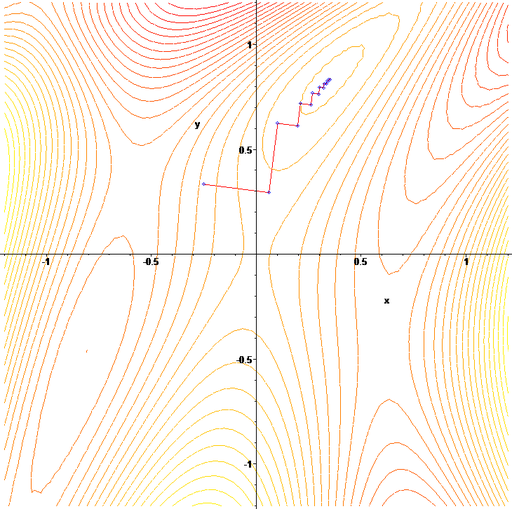
\includegraphics[width=0.9\textwidth]{grad1.png}
      \end{center}
    \end{column}
    \begin{column}{0.49\textwidth}
      \begin{center}
        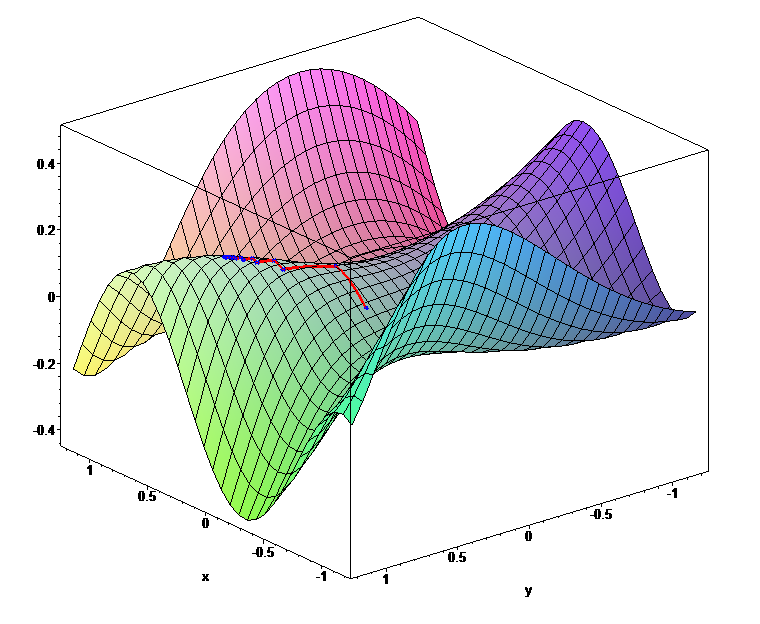
\includegraphics[width=0.9\textwidth]{grad2.png}
      \end{center}
    \end{column}
  \end{columns}
}

\pagestepalt{Stochastic gradient descent}{
  \vspace{-1.1cm}
  Problem: we don't \textbf{have} an explicit function $F$. We're trying to
  do \alert{regression}, right?\pause
  \begin{itemize}
  \item Since $F(\mathbf{x})$ is the loss function, we're trying to
    minimize it over a bunch of observations given parameters
    $\mathbf{w}$.\pause
    \begin{block}{}
      \[F(\mathbf{w}) = \frac{1}{n} \sum^n_{i=1} Q_i(\mathbf{w})\]
    \end{block}\pause
  \item Then our update function becomes:
    \begin{block}{}
      \[\mathbf{w}_{n+1} = \mathbf{w}_n - \gamma \sum^n_{i=1} \nabla Q_i(\mathbf{w}) \]
    \end{block}
    where $\gamma$ is our step size or \alert{learning rate}. \pause
  \end{itemize}
  Then we have an algorithm over observations to estimate the weights\ldots
}

\pagestepalt{Stochastic gradient descent}{
  \ldots which looks like this:\pause
  \begin{block}{(Wikipedia says\ldots though I changed the variable names)\pause}
    \begin{enumerate}
    \item Choose an initial vector of parameters $\mathbf{w}$ and a learning rate $\gamma$.\pause
    \item Repeat until an approximate minimum is obtained.\pause
      \begin{itemize}
      \item Randomly shuffle the examples in the training set.\pause
      \item For $i = 1,2,\ldots,n$ do:
        \begin{itemize}
          \item $\mathbf{w} \Leftarrow \mathbf{w} - \gamma\nabla F_i(\mathbf{w})$
        \end{itemize}
      \end{itemize}
    \end{enumerate}
  \end{block}\pause
  \begin{itemize}
  \item Can pick a ``mini-batch'' instead of instance-by-instance.\pause
    \begin{itemize}
    \item So need to choose learning rate and batch size.\pause
    \end{itemize}
  \item Convergence -- not exactly guaranteed, but very likely.
  \end{itemize}
}

\placard{Part 3: A little more on softmax}

\pagestepalt{Normalization again}{
  \begin{block}{General form of a log-linear model}
      \[P(y|\mathbf{x}) = \text{softmax}(\mathbf{w}_y \cdot \mathbf{x}) = \frac{e^{\mathbf{w}_y \cdot \mathbf{x}}}{Z}\]
  \end{block}\pause
  where $y$ is the class, $\mathbf{w}_y$ is a weight vector
  \alert{specific to that class}, $\mathbf{x}$ is the instance feature
  vector, and $Z$ is the \textbf{normalization constant}.
  \begin{block}{Normalization constant}
    \[Z = \sum_h^Y e^{\mathbf{w}_h \cdot \mathbf{x}}\]
  \end{block}
  where $Y$ is the set of classes.\\
}

\placard{Which means that we need to learn weights \alert{for every class} that represent the relationships between features and classes.}

\pagestepalt{Softmax Normalization}{

% http://tex.stackexchange.com/a/54007
\begin{minipage}[0.8\textheight]{\textwidth}
\begin{columns}[T]
\begin{column}{0.6\textwidth}
\begin{itemize}
	\item<1-> The slowest part of training a neural net LM is softmax normalization
	\item<2-> Why?  Before the softmax layer (final layer) we just have a real number, not a probability\pause
	\item<3-> So we need to know the sum of scores for all possible words being predicted (ie. the normalization constant)
\end{itemize}
\end{column}
\begin{column}{0.4\textwidth}
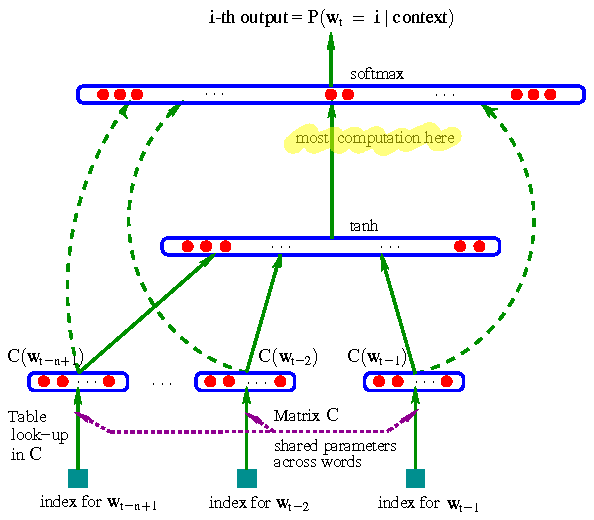
\includegraphics[width=0.8\textwidth]{../images/bengio-etal2003_pg6_image_alt2.pdf}
\end{column}
\end{columns}
\end{minipage}

\pause

\hspace*{-2.5em}%
\begin{minipage}{1.0\textwidth}
\begin{itemize}
	\item<4-> This involves $|V|$ steps, where $|V|$ is the size of the vocabulary
	\item<5-> Typical values of $|V|$ are between 10K to 10M
	\item<6-> We must do this for every word in our training set (eg.\ 1M--1B), every epoch ($>10$)
\end{itemize}
\end{minipage}

}


\pagestepalt{Speeding Up Normalization}{
\begin{itemize}[<+->]
	\item Can we speed up normalization? We can approximate $Z$\,:
	\item \textbf{Class-based Decomposition} works like class-based LMs: first determine prob.\ of a given word's class/POS, then the prob.\ of the specific word \detail{$\mathcal{O} ( \sqrt{|V|} )$}
	\item \textbf{Hierarchical Softmax} extends this idea to a fully binary-branching hierarchy of the vocabulary (like an ontology) \detail{$\mathcal{O} (\log_2(|V|) ) $ }
	\item \textbf{Noise Contrastive Estimation} (NCE) disposes with MLE (in Softmax).  Instead, a binary classifier is learned: observed training data vs.\ artificially generated noise.  word2vec's negative sampling is a simplified version. \detail{$\mathcal{O} (1) $}
	\item \textbf{Self Normalization} ensures that the normalization constant $Z$ is close to one. Slow for training, fast for test-time queries
\end{itemize}
}

\pagestepalt{Rube Goldberg Network}{
  \vspace{-0.7cm}
\begin{center}
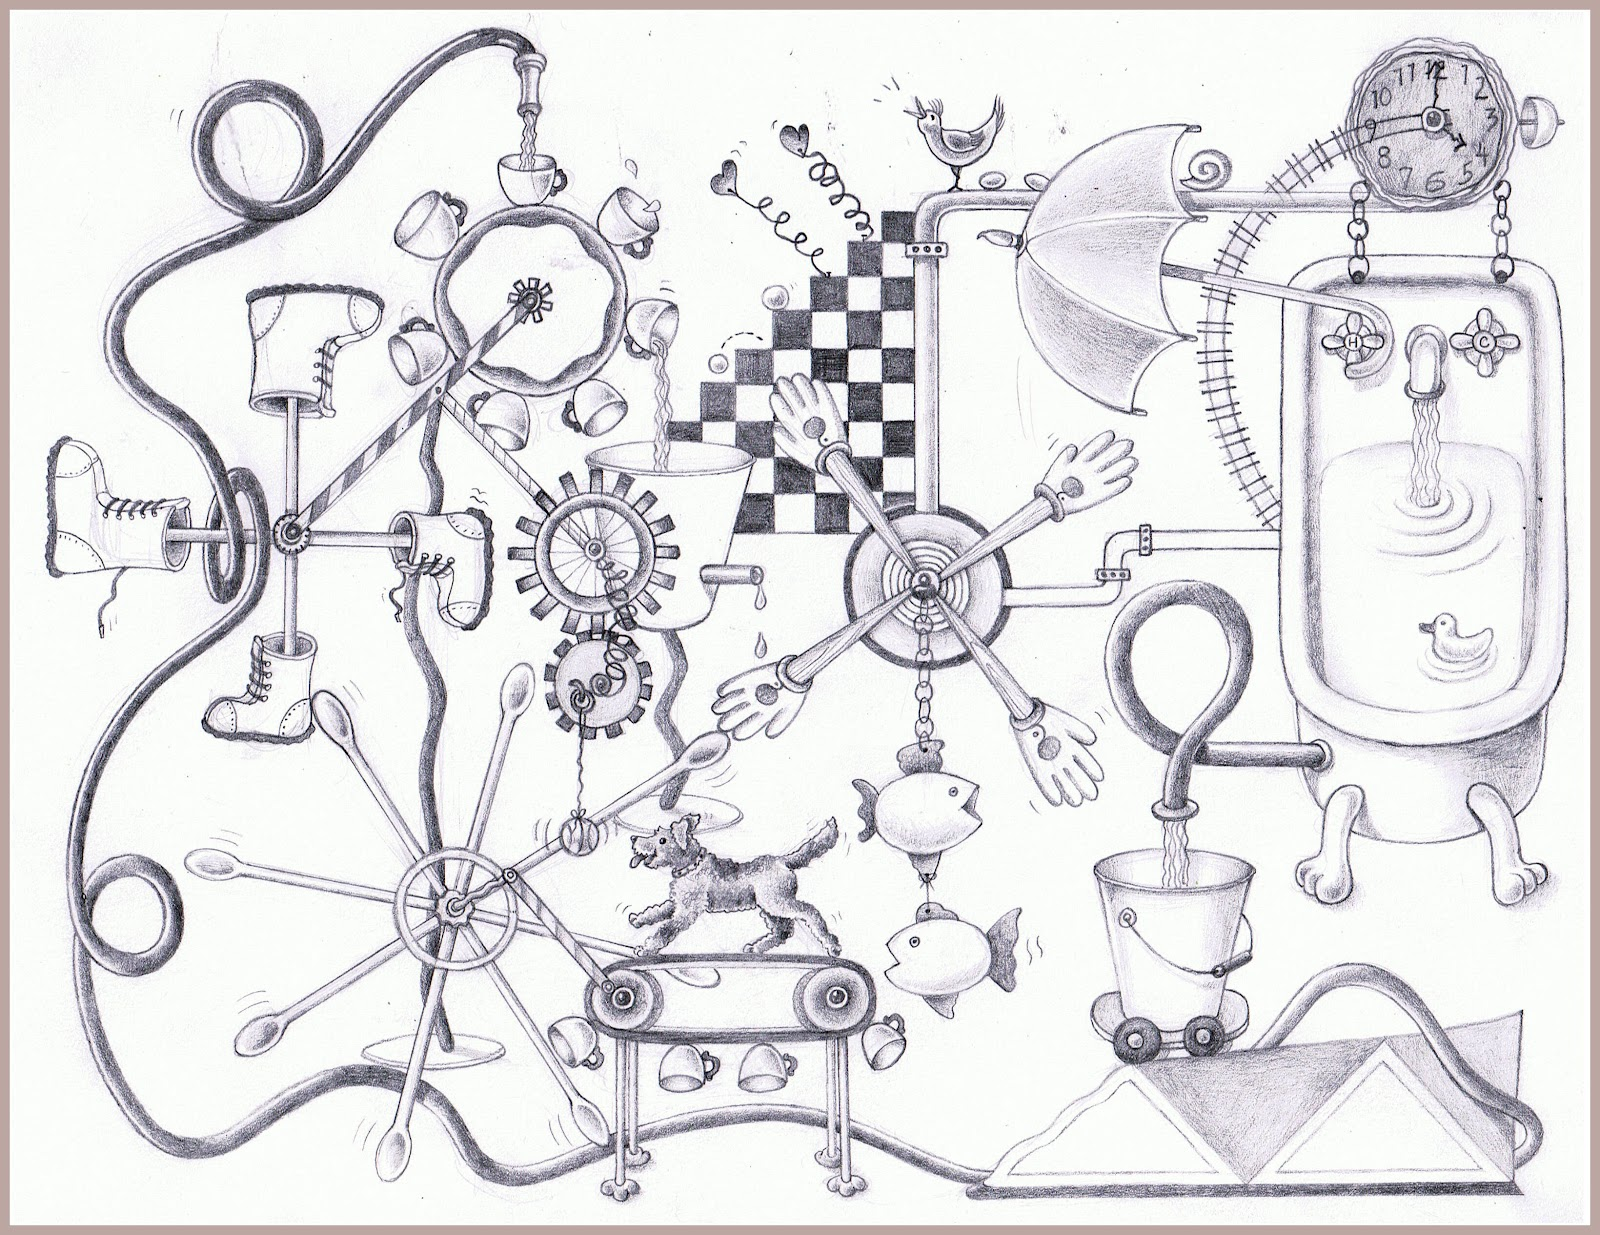
\includegraphics[width=0.85\textwidth]{../images/rube_goldberg_machine.jpg}
\end{center}
}

\pagestepalt{Further Reading}{
\vspace{-1ex}
\textbf{Overviews}: \\[0.5em]
\begin{minipage}{1.1\textwidth}
\begin{tiny}
\begin{itemize}
	\item \url{https://www.reddit.com/r/MachineLearning/comments/44bxdj/scrn\_vs\_lstm/czp4hqr/}
	\item \url{https://colah.github.io/posts/2015-08-Understanding-LSTMs/}
	\item \url{https://medium.com/@shiyan/understanding-lstm-and-its-diagrams-37e2f46f1714}
	\item \url{http://deeplearning.net/tutorial/lstm.html}
	\item \url{http://arxiv.org/abs/1412.3555}
	\item \url{https://www.tensorflow.org/versions/master/tutorials/recurrent/index.html\#recurrent-neural-networks}
	\item \url{http://keras.io/layers/recurrent/}
	\item \url{https://drive.google.com/open?id=0B-aFax-9-qt3Sllodkpmc1M0MUk}
	\item \url{https://en.wikipedia.org/wiki/LSTM}
\end{itemize}
\end{tiny}
\end{minipage}

\vspace{0.5em}
\textbf{Original Papers}:
\begin{tiny}
\begin{description}
	\item[SRN] Elman, Jeffrey L. 1990. \href{http://citeseerx.ist.psu.edu/viewdoc/summary?doi=10.1.1.28.9476}{Finding Structure in Time}. \textit{Cognitive Science} 14.179--211.
	\item[LSTM] Hochreiter, Sepp, and J\"{u}rgen Schmidhuber. 1997. \href{http://deeplearning.cs.cmu.edu/pdfs/Hochreiter97_lstm.pdf}{Long Short-Term Memory}. \textit{Neural Computation} 9.1735--1780.
	\item[GRU] Kyunghyun Cho, Bart van Merri\"{e}nboer, \c{C}a\u{g}lar G\"{u}l\c{c}ehre, Fethi Bougares, Holger Schwenk, and Yoshua Bengio. 2014. \href{https://arxiv.org/abs/1406.1078}{Learning phrase representations using RNN encoder-decoder for statistical machine translation}. In \textit{Proceedings of the Empiricial Methods in Natural Language Processing (EMNLP 2014)}.
\end{description}
\end{tiny}
}


%% \pagestepalt{Training Neural Networks}{
%% \begin{itemize}
%% 	\item At a high level, the weights in a neural net are set by means of the blame game -- whenever it guesses incorrectly, change the weights that were the most responsible for making that guess
%% 	\pause
%% 	\item Whenever the network guesses a training instance correctly, don't change anything
%% 	\pause
%% 	\item The weights are usually trained by a form of the gradient descent optimization algorithm
%% 	\item The gradients are calculated by error \textbf{backpropagation}
%% 	\item First, do a normal forward pass through the network, to determine the \textbf{error/loss} (how different the output was from the `correct' answer)
%% 	\item Then, do a backwards pass (end to start), changing the weights to minimize errors
%% \end{itemize}
%% }


%% \pagestepalt{Tips \& Tricks (discussed in class)}{
%% \begin{itemize}
%% 	\item Network depth
%% 	\item Layer size
%% 	\item Dropout
%% 	\item Early stopping
%% 	\item Optimizers
%% 	\item Learning rate
%% \end{itemize}
%% \vspace{5.0em}
%% \teeny{See also \url{https://www.linkedin.com/pulse/what-i-learned-from-deep-learning-summer-school-2016-hamid-palangi}}
%% }



\end{document}
